\documentclass[11pt]{article}
\usepackage{basecommon}
\usepackage[margin=1.5in, top=1in]{geometry}
\usepackage[backend=bibtex, natbib=true, autocite=superscript, style=authoryear-ibid]{biblatex}
\usepackage{hyperref}
\usepackage{url}
\usepackage{lineno}
\usepackage{graphicx}
\usepackage{tikz}
\usetikzlibrary{positioning}
\tikzset{
  treenode/.style = {shape=rectangle, rounded corners,
                     draw, align=center,
                     top color=white, bottom color=blue!20},
  root/.style     = {treenode, font=\Large, bottom color=red!30},
  env/.style      = {treenode},
  result/.style	={treenode, font=\Large, top color=blue!20, bottom color=blue!20}
}
\urldef{\JSBChorales}\url{http://www-etud.iro.umontreal.ca/~boulanni/icml2012}
\addbibresource{../ch1/citations_annotated.bib}
\usepackage{setspace}
\doublespacing
\linenumbers
\title{Chapter 2 (DRAFT - 3/1/16)}
\author{Hugh Zabriskie}
\date{7 March 2016}
\begin{document}
\maketitle{}

\section{Motivation for the harmonization task}

The task explored in this paper is the generation of four-part counterpoint given a chorale melody. J.S. Bach's collection of over 300 chorale harmonizations is used as the dataset because it remains today one of the finest examples of four-part counterpoint. Each harmonization is a complex solution, satisfying a variety of voice leading and cadential constraints, as well as innumerable other conventions of musical style. Chorale harmonization is therefore a fundamentally difficult computational task. Initial observations might suggest a rule-based approach to this task, whereby musical constraints are computationally encoded and only harmonizations that satisfy them are generated. However, a purely rule-based approach is rendered impractical by a couple important factors. One is the sheer number of conventions that would need to be encoded, each with a varying level of specificity and precedence with respect to the other encoded conventions. Determining precisely what those conventions would be is an even more difficult problem, since many chorale constraints are vaguely defined or flexible in application. Another reason for avoiding a rule-based approach is that an infinite quantity of harmonizations exist that satisfy any given chorale melody. The goal is not to simply produce satisfying harmonizations, but to \textit{approximate} Bach's harmonization as closely as possible. In contrast, a "learning" model updates its parameters to capture the complex correlations and patterns it discovers in the training set of harmonizations. Applying those parameters to a new chorale melody will then yield a predicted harmonization, and its predictions will directly reflect (and only reflect) the harmonizations the model was trained upon.
  
\section{Literature Review}

\subsection{Previous Work}

\citet{hild1992harmonet} presented the first effective neural network approach for harmonizing chorales, generation harmonizations on the level of an "improvising organist" (p. 272). The task decomposed into three subtasks, each learned by a neural net. A harmonic skeleton is first created by sweeping through the chorale melody and determining a harmony for each beat, where harmony is represented by a unique figured bass notation. For each time step $t$, the network takes an input a window of information, including the harmonies chosen in the interval$[t-3, t-1]$ and the melody pitches in the interval $[t-1, t+1]$. The resulting harmonic skeleton is passed to another network to generate a chord skeleton, which selects the inner voices based on the input figured bass, and a final network adds ornamental eighth notes to restore passing tones between chords. Although, HARMONET demonstrated strong success, the model used external "chorale constraints" \citep[p.~271]{hild1992harmonet} in constructing the chord skeleton in order to avoid unfavorable chord structures. The models presented in this paper attempt to learn the task of harmonization without any form of manual intervention in the network's learning process. \\

Substantial work has been done in the field of music generation using RNNs and LSTMs that demonstrates their ability to learn complicated musical structures and relate temporally distant events, particularly in the realm of melodic generation. \citet{petri1995bebop} developed a neural network that generates a jazz bebop melody over series of chord changes. The network achieves melodic continuity by using a "target-note technique", where the end of a previous melody segment and the present chord are used to predict the next melodic pattern at time $t+1$, while the following chord at time $t+2$ is use to optimize of the melodic pattern, thereby smoothing the melodic transitions over chord changes. \citet{eck2002structure} improved on the results of \citet{mozer1994neural}, who used RNNs to compose melodies with chordal accompaniment but found the resulting music lacked larger thematic and phrase structure. They attributed Mozer's results to the "vanishing gradients" problem (described briefly in chapter 1) and then trained LSTMs to first generate the chordal structure and use that as a input to the LSTMs that generates a blues-style melody with promising results. \citet{franklin2006jazz} also used LSTMs (two inter-recurrent networks) to compose jazz melodies over a chord progression, training the networks on a dataset of well-known jazz standard melodies. \\

Research specifically on models for the Bach chorales have seen a variety of approaches. \citet{allan2005harmonising} generated a dataset of the chorales by transposing each chorale to C major or C minor and then sampling every quarter note, now available at \JSBChorales. They trained Hidden Markov Models (HMMs) on the data to model chorale harmonization, creating a probabilistic framework for deciding the most likely choice of alto, tenor, and bass notes to complement the melody in each time frame. More recent work has focused on music \textit{generation} models rather than completive models. Boulanger-Lewandowski et. al. (2012) used this version of the dataset, along with multiple other corpuses, to make a comprehensive survey of music generation models that performed next-step prediction for all voices. Based on log-likelihood and overall accuracy on the test data, a specific flavor of RNNs was found to be most effective on all corpuses used in the study. Other studies have sought to "re-construct" chorales using more sophisticated neural models (Liu, 2014), including a large-scale survey of polyphonic music modeling that evaluated the performance of eight LSTM variants \citet{greff2015lstm}. Both previous papers mentioned highlight the use of RNNs and LSTMs as effective models because of their ability to learn temporal dependencies within polyphonic music (i.e. how distant musical events can be related). Notably, the latter found the "vanilla", unmodified LSTM equally effective as the other variants \citep[p.~7]{greff2015lstm}, so this architecture was chosen for this study.

My approach consists of applying a variety of non-neural and neural models to the task of chorale harmonization. Recent harmonization and generative models (\cite{allan2005harmonising}; \cite{kaliakatsos2014}; \cite{greff2015lstm}) relied on a dataset that includes only pitch information about each time step, and the objective was in all cases next step pitch prediction. My goal was to extract a new set of features from Bach's chorales and examine how those features improved or worsened model performance. Moreover, the objective was to learn a series of musical processes that decide the harmony at each time step that include both harmonic analysis and note selection. I chose this approach to mimic the decisions a musician would make today in harmonizing a chorale.

\section{Methods}

A corpus of chorales was gathered in MIDI format (\cite{greentree2005}) through the \textsc{music21} library. \textsc{music21} is maintained by Professor Michael Scott Cuthbert at MIT and provided the essential tools for parsing musical scores and musical feature extraction. The code developed for this paper builds off of the built-in \textsc{music21} objects that represents the hierarchy of musical components introduced in Chapter 1. From this dataset, 326 4-voice chorales were gathered, and some manual cleaning was then performed to correct mistakes in the musicXML format related to key signatures and clear mistakes in notation. Each chorale was then sampled at each quarter-note time frame so that rhythmic variation would be factored out. Like modern church hymns, Bach's chorales are very uniformly structured, with harmonic progressions that change on each beat. Moving eighth notes typically help with voice leading rather than define the harmony so quarter-note sampling is a reasonable approach and has been used in several other studies (\cite{hild1992harmonet}; \cite{madsen2002}; \cite{kaliakatsos2014}).

\subsection{Harmonization subtasks}

In order to evaluate a model's ability to learn different aspects of the harmonization process the decision process was broken into 4 sequential subtasks. For each melody note in each chorale, the following target outputs were extracted.

\begin{enumerate}
\item \textit{Roman numeral}. The model first decided the general harmonic function by selecting a Roman numeral per Roman numeral analysis. This decision holds the most importance since it decides what notes are allowed for the alto and tenor voices.
\item \textit{Inversion}. The chord inversion provides additional harmonic information since, for example, a \rom{1}$^6$ harmony has different implications about future harmonies than a \rom{1} chord in root position. The inversion also implies the pitch class of the bass voice.
\item \textit{Alto}. The alto voice is then selected as the first inner voice. There is no reason for selecting the alto voice before the tenor voice since both function similarly as inner voices that support the harmony decided in the previous subtasks.
\item \textit{Tenor}. Selection of the tenor voice completes the harmonization.
\end{enumerate}

Mathematically, the algorithm should take as input the chorale, represented a sequence of notes, and it should output a corresponding sequence of 3-voice chords that represent the alto, tenor, and bass voices. We will say we have $m$ data points with $n$ features, and $Y$ output classes.
\begin{itemize}
\item $\boldX \in V^{m \times n}$ is our input data
\item $\boldY \in Y^m$ is our output data for a given subtask
\item The objective is to approximate the complex function $f: \boldX \to \boldY$
\end{itemize}

In order to generate the correct Roman numeral analysis for the first two subtasks, I relied on a combination of \textsc{music21}'s \texttt{roman} module for initial analysis followed by substantial manual correction due some incomplete functionality in the analysis module. The alto and tenor voices were extracted as MIDI note values. \\

\begin{figure}[h]
\begin{center}
\caption{\textbf{Sequence of harmonization subtasks.}}
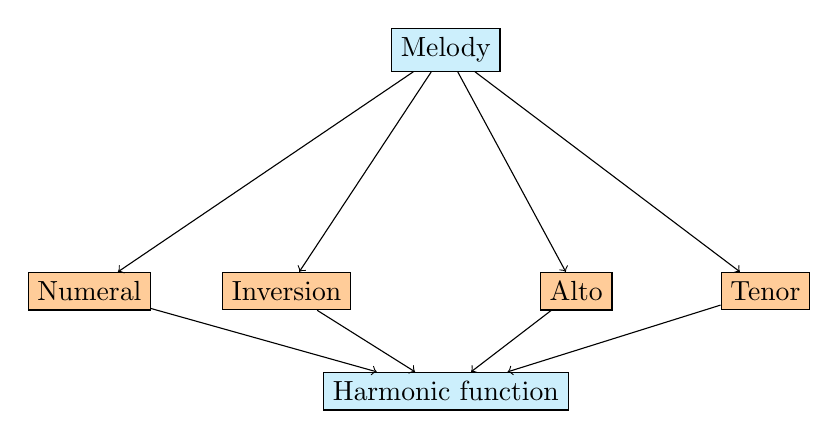
\begin{tikzpicture}
  [
    grow                    = down,
    sibling distance        = 6em,
    level distance          = 4em,
    edge from parent/.style = {draw, -latex}
  ]
  \begin{scope}[end/.style={rectangle,draw,fill=cyan!20},
  			env/.style={rectangle,draw,fill=orange!40}, node distance=1in]
  \node [end] (mel) {Melody};
  \node [end] (el) [below=1.5in of mel] {Harmonic function};
  \node [env] (a) [below left=1in and 1.2in of mel] {Numeral} edge [->] (el);
  \node [env] (b) [below left=1in and 0.2in of mel]{Inversion} edge [->] (el);
  \node [env] (c) [below right=1in and 0.5 of mel] {Alto} edge [->] (el);
  \node [env] (d) [below right=1in and 1.1in of mel] {Tenor} edge [->] (el);
  \path[->] (mel) edge node {} (a);
  \path[->] (mel) edge node {} (b);
  \path[->] (mel) edge node {} (c);
  \path[->] (mel) edge node {} (d);
  \end{scope}
\end{tikzpicture}
\end{center}
\end{figure}


\subsection{Feature Extraction}

In order to learn each of these subtasks, the following information was extracted for each melody note in each chorale.

\begin{enumerate}
\item The number of sharps in the key signature. Flats were given negative values.
\item The mode (i.e. major or minor) of the chorale.
\item The time signature of the chorale.
\item Beat strength, or metrical accent. A 4/4 measure would be assigned the following pattern: [ 1.0, 0.25, 0.5, 0.25 ]
\item The presence of a fermata - a binary feature indicating a cadence.
\item Number of beats until the next fermata.
\item Number of measures until the end of the chorale.
\item The melody pitch, encoded as a MIDI value. A search across all chorales indicated that each voice had a well-defined pitch range, verified by \citet{madsen2002}: 
\begin{itemize}
\item \textit{soprano}: [60, 81]
\item \textit{alto}: [53, 74]
\item \textit{tenor}: [48, 69]
\item \textit{bass}: [36, 64]
\end{itemize}
\item The interval to the previous melody note.
\item The interval to the next melody note.
\item The Roman numeral for the previous time step.
\item The inversion for the previous time step.
\end{enumerate}

Features 11 and 12 were used only for Oracle experiments and demonstrating the potential of RNNs, discussed later in Chapter 3. \\

The Python script used to preprocess the chorales (see wrangle.py in Appendix B) \footnote{There will be an Appendix B that contains the most important code for the project.} extracts the above features from each time step of each chorale, and stores the generated training and tests in an HDF5 file. For baseline models, the extracted data was fed as input to another Python script that performed classified learning using models from the\textsc{scikit-learn} module. For neural models, the data was fed into Lua scripts that use the scientific computing framework Torch to construct models and training on supervised classification tasks.


\section{Baseline models}

Due to unique classification problems chosen for this paper, previous computational research on the chorales does not provide any adequate baseline models. Baseline models are important because they provide a basis for comparison when evaluating other models. As the complexity of the model changes and the features are added or removed, it is important to have a metric to compare against to see how those changes improved or worsened the results. In classification problems, a crude baseline model can be achieved by choosing the class with the most observations and using that class as the result for all predictions. TABLE 2 lists the baseline frequencies for the most common classes for each subtask. I also trained three other classifiers to get a sense of the complexity of each subtask. These classifiers are described below: \\
\textit{Multiclass logistic regression} was introduced in Chapter 1 as a generalization of the binary classification system of logistic regression. Despite its name, this regression is a linear model. The objective is to minimize the following cost function, given the learned parameters $\theta$.
$$ J(\theta) = -\frac{1}{m} \sum_{i = 1}^{m} \sum_{k  = 1}^{K} \{ \boldy^{(i)} = k \} \log \Big( \frac{ \exp(a_{ik}) } { \sum_j \exp(a_{ij}) } \Big) $$
Where $m$ is the number of examples, $k$ is the number of classes, and $a_{ik}$ is the "activation" function $\theta^{(k)T} x^{(i)}$, denoted for the $i$th example and the $k$th class.

\textit{Multinomial naive Bayes} generalizes the naive Bayes algorithm for multi-class data, and it makes the "naive" assumption of independence between every pair of input features. The assumption therefore states that, given the input vector $\boldx$ and the class $c \in [1, K]$
$$P(\boldx | c) = P(\boldx_1, \boldx_2, \ldots, \boldx_n | c) = \prod_{i=1}^{n} P(\boldx_i | c)$$
And based on that assumption, this baseline classifier the predicted output class is decided by
$$P(c | \boldx) = \frac{ P(\boldx | c) P(c) }{ \sum_j P(\boldx | C_j) P(C_j) } = \frac{ \prod_i P(\boldx_i | c) P(c) }{ \sum_j \prod_i P(\boldx_i | C_j) P(C_j) }$$\\

\textit{Random forests} are a powerful supervised learning technique that involves classification based on a the majority vote of a series of decision trees. Each tree is initialized with data from a random subset of features and then is trained on the data by sampling with replacement. This randomness is known to be highly effective in preventing overfitting on training data, and random forests generalize well on weaker datasets where one or more training examples do not strongly suggest differences between classes \citep[p.~18]{breiman2001}.

The results for each baseline model are described in Table 1. \\

\begin{table}[h]
\begin{center}
\caption[Table caption text]{\textbf{Baseline model test accuracy on harmonization subtasks.}}
\begin{tabular}{l | c c c c}
Classifier & Numeral & Inversion & Alto & Tenor \\ \hline
Multi-Class Logistic & 31.61\% & 59.76\% & 37.55\% & 37.86\% \\
Multinomial Naive Bayes & 27.44\% & 56.66\% & 35.06\% & 34.40\% \\
Random Forests & 49.29\% & 61.64\% & 49.44\% & 45.43\% \\
\end{tabular}
\end{center}
\end{table}

\begin{table}[h]
\begin{center}
\caption[Table caption text]{\textbf{Most common class frequency.}}
\begin{tabular}{l | c c}
Subtask & Training Set & Test Set \\ \hline
Numeral & 19.2\% & 19.2\% \\
Inversion & 55.5\% & 57.6\% \\
Alto & 15.7\% & 14.6\% \\
Tenor & 15.6\% & 15.5\%
\end{tabular}
\end{center}
\end{table}


\subsection{GCT Algorithm}

While Roman numeral analysis has been the traditional method for describing harmony in the Chorales, it presents issues for statistical learning. Roman numeral classification mainly depends on the key signature, but also requires the context of the preceding harmonies. For example, a D major chord in a C major chorale might be labelled as a \rom{2} or \rom{5}/\rom{5} depending on whether a modulation to D major had occurred or whether the preceding harmonies indicate that it functions as a secondary dominant. During training, finding two or more inputs that suggest a D major chord but are labeled differently can cause confusion in learning, particularly since in non-recurrent models there is no sense of context about other local harmonies. Roman numeral chord labeling can be further complicated by the presence of non-chord tones, which makes, for example, differentiating \rom{4}$^6$ and \lrom{2}$^7$ chords computationally difficult.\\

The general chord type (GCT) representation provides an idiom-independent solution to encoding harmony that assigns a unique encoding to each chord, regardless of context \citep{2014gct}. To encode a chordal harmony, the GCT algorithm takes as input the chord to be encoded, a pitch scale that describes the tonality, and a binary "consonance vector" $\boldv$ such that $\boldv[n] = 1$ if an interval of $n$ semitones is considered consonant for $0 \leq n \leq 11$. In this study, I chose $\boldv = [1, 0, 0, 1, 1, 1, 0, 1, 1, 1, 0, 0]$.  GCT then constructs an ordering of the chord pitches that maximizes the consonant intervals between all pairs of pitches. The remaining notes that create dissonant intervals are labeled as "extensions". The algorithm outputs a encoding of the form [root, [base, extensions]], where root is the pitch class of the chord root relative to the tonic, and the base is the ordering of maximal consonance. I adapted the algorithm to also output the degree of inversion, where 0 represents root position, 1 represents first inversion, and so on. Figure 2 demonstrates an application of the GCT algorithm to a tonal harmonic progression, comparing the Roman numeral analysis with the GCT encoding. The base [0, 4, 7] encodes a major triad, while [0, 3, 7, 10] encodes a minor seventh chord.

\begin{figure}[h]
\begin{center}
\caption{Example of the GCT and Roman numeral notation.}
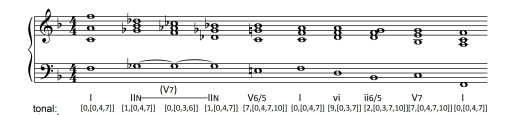
\includegraphics[scale=0.7]{GCT}
\end{center}
\end{figure}

In comparison with a Roman numeral analysis dataset compiled by David Temperley, GCT labeled 92\% of the chords accurately, of which about 1/3 of mislabeled chords were diminished sevenths - excusable because each note in the chord can function as the root \citep{2014gct}. In order to minimize duplicate encodings, I implemented the following policies, partially drawn from suggestions by the original authors.
\begin{enumerate}
\item For dyads, prefer an interval of a 5th over a 4th, and an interval of a 7th over a 2nd.
\item Preference encodings where all intervals are larger than a major 2nd. This heuristic preferences a minor 7th or a major chord with an added 6th, and generally more evenly spaced encodings.
\item If more than one encoding remains, choose randomly.
\end{enumerate}

The GCT algorithm was incorporated into a newly generated dataset for the chorales by replacing the numeral and inversion subtasks in $\boldY$ with the new root, base, and inversion subtasks. The root subtasks establishes the chord root, while the remaining chord structure is decided by the base. As in Roman numeral analysis, the inversion implies which chord tone is assigned to the bass. As well, the new dataset classified the tenor and alto voices by their distance from the tonic pitch, instead of encoding MIDI values directly, in order to make the decision key-independent and reduce the output class space to a maximum of 12 classes (for the 12 chromatic intervals).\\

The same baseline models were used to evaluate the new subtasks. In both cases, there were 293 chorales in the training set, and 33 chorales in the test set.

\begin{table}[h]
\begin{center}
\caption[Table caption text]{\textbf{Baseline model test accuracy with new GCT subtasks.}}
\begin{tabular}{l c c c c c}
Classifier & Root & Base & Inversion & Alto & Tenor \\ \hline
Multi-Class Logistic & 58.29\% & 56.09\% & 67.06\% & 38.22\% & 36.33\% \\
Multinomial Naive Bayes & 48.19\% & 50.43\% & 62.66\% & 34.73\% & 31.65\% \\
Random Forests & 63.71\% & 59.72\% & 69.73\% & 47.22\% & 46.81\% \\
\end{tabular}
\end{center}
\end{table}

\begin{table}[h]
\begin{center}
\caption[Table caption text]{\textbf{Majority class frequency (MCCF), with GCT subtasks.}}
\begin{tabular}{l | c c}
Subtask & Training Set & Test Set \\ \hline
Root & 28.5\% & 28.0\% \\
Base & 49.5\% & 49.9\% \\
Inversion & 63.9\% & 65.5\% \\
Alto & 22.6\% & 23.7\% \\
Tenor & 20.3\% & 22.0\%
\end{tabular}
\end{center}
\end{table}

\begin{figure*}[ht]
\caption{ Harmonization subtask accuracy comparison }
\centerline{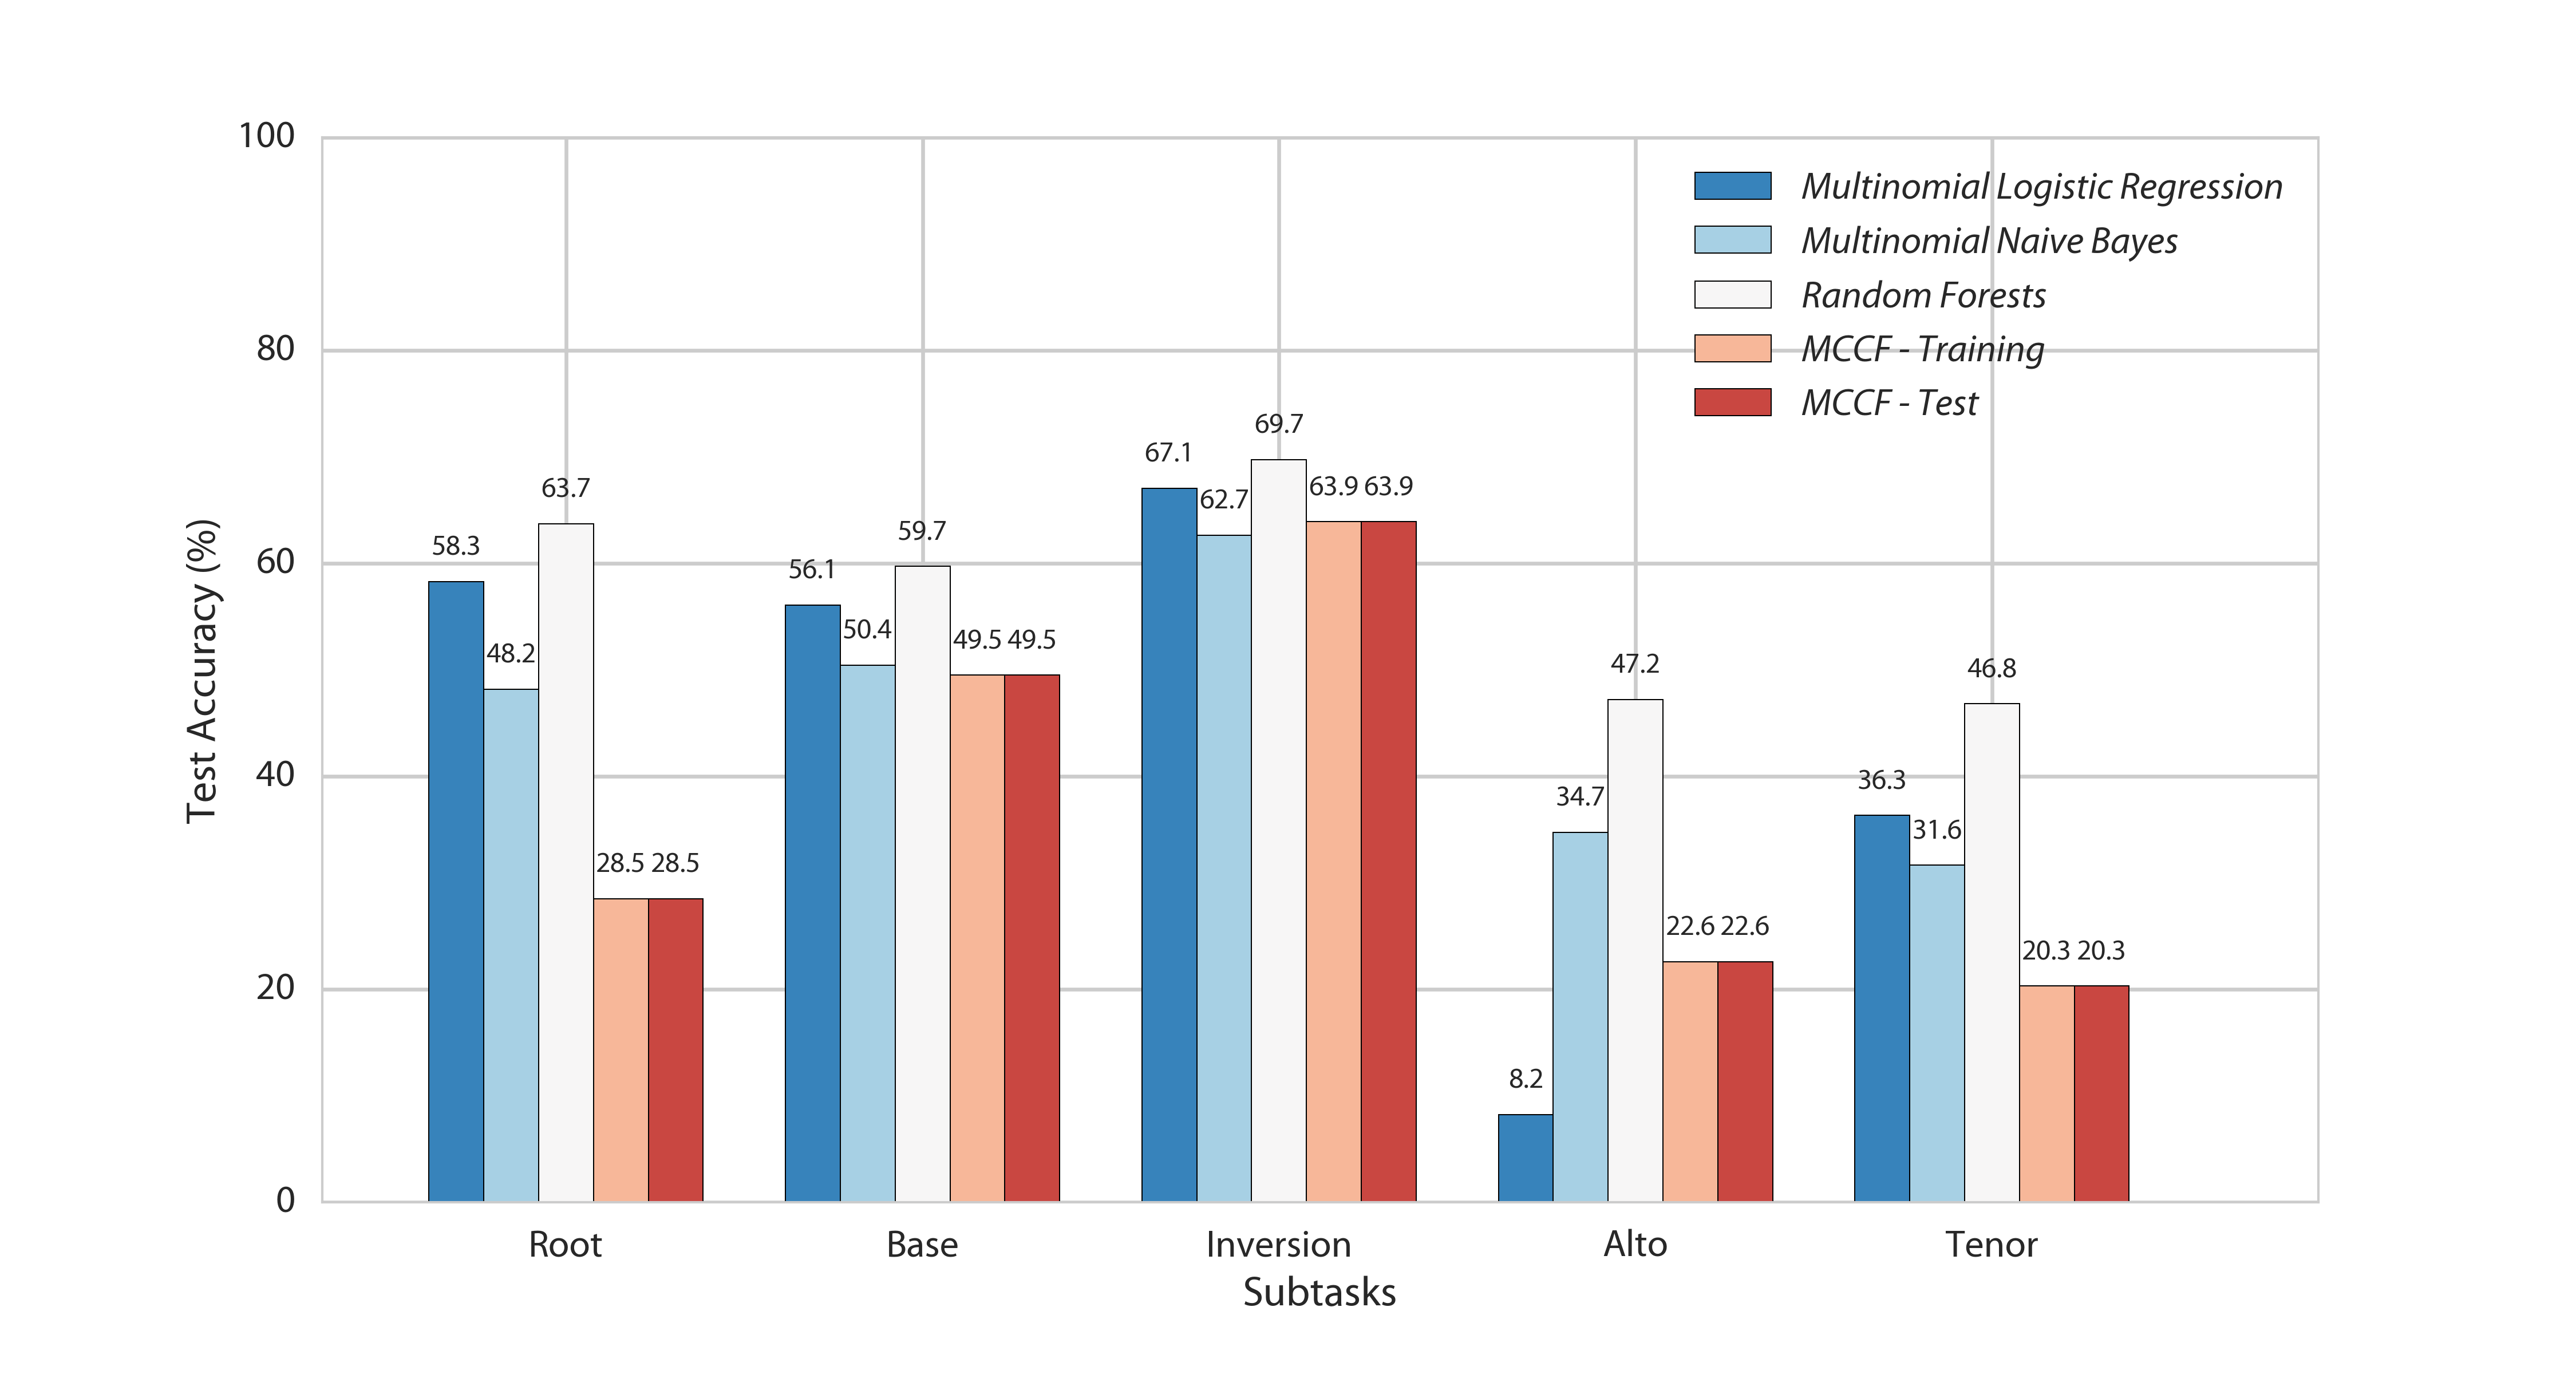
\includegraphics[scale=0.5]{subtasks}}
\end{figure*}



Figure 3 provides a visual comparison of baseline model performance across all harmonization subtasks. For all subtasks, a majority of the multinomial models outperformed the MCCF baselines. In particular, Random Forests consistently outperformed the other models, with a 35\% increase in accuracy over the MCCF baseline for the root subtask. However, the multinomial models struggled to perform above the MCCF baselines  for both the base and inversion subtasks, which appears correlated with a high predominance of a single class in the dataset. This points to an issue with an imbalance class distribution in the data. Of the 133 output classes for the GCT base subtask, the most common class is associated with 50\% of all observations in entire dataset (this happens to be the major triad), and the top 3 most frequent classes account for 77\% of all observations. Consequently, the vast majority of output classes are observed too infrequently in the training data to be classified accurately in the test data. Imbalanced data is a widely recognized phenomenon in data mining that is comprehensively detailed in \citet{sun2009classification}. The significant advantage achieved using random forests can potentially be explained by its known effectiveness at classification when one or more observations is not sufficient to generally distinguish a class \citep[pg.~18]{breiman2001}.

\printbibliography



\end{document}